\documentclass[12pt,a4paper]{article}
\usepackage[utf8]{inputenc}
\usepackage[T1]{fontenc}
\usepackage{amsmath}
\usepackage{amsfonts}
\usepackage{amssymb}
\usepackage{amsthm}
\usepackage{graphicx}
\usepackage{subfigure}
\usepackage{float}
\newtheorem*{lemma}{Lemma}
\newtheorem*{theorem}{Theorem}
\newtheorem*{corollary}{Corollary}
\newtheorem*{prf}{\textbf{Proof}}
\usepackage{caption}
\DeclareMathOperator{\n}{\nabla}
\DeclareMathOperator{\E}{\mathrm{E}}
\DeclareMathOperator{\xyz}{\textbf{numpy.random.normal()}}
\title{CS331-HW7-Lukang-Sun}
\begin{document}
	\maketitle
	\paragraph{p1.}
	(i) the method is the same as the one described in class, but with different variance parameters.
	\newline
	(ii)
	\begin{lemma}
		 Assume that functions $f_{i}$ are convex and $L_{i}$-smooth for all i. Let $\mathcal{C}_{i} \in \mathbb{B}^{d}(\omega_i)$ for all i. Suppose that $\alpha \leq \frac{1}{\omega_{max}+1} .$ Let $h=\left(h_{1}, h_{2}, \ldots, h_{n}\right) \in \mathbb{R}^{d} \times \mathbb{R}^{d} \cdots \times \mathbb{R}^{d}=\mathbb{R}^{n d}$ and define $\sigma: \mathbb{R}^{n d} \rightarrow[0, \infty)$ and $\sigma^{k}$ by
		$$
		\sigma(h)=\frac{1}{n} \sum_{i=1}^{n}\left\|h_{i}-\nabla f_{i}\left(x^{\star}\right)\right\|^{2} \quad \sigma^{k} \stackrel{\text { def }}{=} \sigma\left(h^{k}\right)=\frac{1}{n} \sum_{i=1}^{n}\left\|h_{i}^{k}-\nabla f_{i}\left(x^{\star}\right)\right\|^{2}
		$$
		Then for all iterations $k \geq 0$ of Algorithm 19 (with different variance parameters) we have
		$$
		\begin{aligned}
			\mathrm{E}\left[g^{k} \mid x^{k}, h^{k}\right] &=\nabla f\left(x^{k}\right), \\
			\mathrm{E}\left[\left\|g^{k}-\nabla f\left(x^{\star}\right)\right\|^{2} \mid x^{k}, h^{k}\right] & \leq 2 \underbrace{\left(\max(L_i(1+\frac{2\omega_i}{n}))\right) }_{A} D_{f}\left(x^{k}, x^{\star}\right)+\underbrace{\frac{2 \omega_{max}}{n}}_{B} \sigma^{k}, \\
			E\left[\sigma^{k+1} \mid x^{k}, h^{k}\right] & \leq 2 \underbrace{\alpha L_{\max }}_{\tilde{A}} D_{f}\left(x^{k}, x^{\star}\right)+\underbrace{(1-\alpha)}_{\tilde{B}} \sigma^{k} .
		\end{aligned}
		$$
	\end{lemma}

	\begin{proof}
		for simplicity, I use $\E\left[\cdot\mid k\right]$ to denote $\E\left[\cdot\mid \mathcal{F}_k\right]$.$g^k=\sum_i \mathcal{C}_i(\nabla_i(x^k)-h_i^k)+\sum_i h^k_i$,
		We only prove the second and the third equality, the first one is trivial.
		\begin{equation}
			\begin{aligned}
			&\E\left[||g^k-\nabla f(x^{\star})||^2\mid k\right]=\E\left[||g^k-\nabla f(x_k)||^2\mid k\right]+||\nabla f(x_k)-\nabla f(x^{\star})||^2\\
					&\leq\frac{1}{n^2}\sum_i\omega_i(2||\nabla f_i(x_k)-\nabla f_i(x^{\star})||^2+2||\nabla f_i(x^{\star}-h_i^k)||^2)+\frac{1}{n}\sum_i2L_i D_{f_i}(x^k,x^{\star})\\
					&\leq \frac{2\omega_{max}}{n}\sigma^k+\max(2L_i(1+\frac{2\omega_i}{n}))D_f(x^k,x^{\star}),
			\end{aligned}
		\end{equation}
	the second inequality is due to the independence of each $\mathcal{C}_i$.
	\begin{equation}
		\begin{aligned}
			&\E\left[\sigma^{k+1}\mid k\right]=\frac{1}{n}\E\left[||h_i^k+\alpha m_i^k-\nabla f_i(x^{\star})||^2\mid k\right]
		\end{aligned}
	\end{equation}
	if we choose $\alpha\in (0,\frac{1}{\omega_{max}+1}]$, then we have for each index $i$,
	\begin{equation}
		\begin{aligned}
			&\E\left[||h_i^k+\alpha m_i^k-\nabla f_i(x^{\star})||^2\mid k\right]\\
			&= ||h^k_i-\nabla f_i(x^{\star})||^2+2\alpha \langle \nabla f_i(x^k)-h_i^k,h^k_i-\nabla f_i(x^{\star})\rangle+\alpha^2(\omega_i+1)||\nabla f_i(x^{\star})-h_i^k||^2\\
			&\leq ||h_i^k-\nabla f_i(x^{\star})||^2+\alpha(2\langle \nabla f_i(x^k)-h^k_i,h^k_i-\nabla f_i(x^{\star})\rangle+||\nabla f_(x^k)-h^k_i||^2)\\
			&=||h^k_i-\nabla f_i(x^{\star})||^2+\alpha(||\nabla f_i(x^k)-\nabla f_i(x^{\star})||^2-||h^k_i-\nabla f_i(x^{\star})||^2)\\
			&\leq (1-\alpha)||h_i^k-\nabla f_i(x^{\star})||+2\alpha L_iD_{f_i}(x^k,x^{\star}),
		\end{aligned}
	\end{equation}
	take summation, we finally get
	\begin{equation}
		\E\left[\sigma^{k+1}\mid k\right]\leq (1-\alpha)\sigma^k+2\alpha L_{max}D_f(x^k,x^{\star}).
	\end{equation}
	\end{proof}
	(iii)
	\begin{corollary}
		Assume that $f_{i}$ is convex and $L_{i}$-smooth for all $i \in[n]$ and $f$ is $\mu$-convex. If the stepsizes satisfy
		$$
		\alpha \leq \frac{1}{\omega_{max}+1}, \quad \gamma \leq \frac{1}{\max_i(\left(1+\frac{2 \omega_i}{n}\right) L_{i})+M L_{\max } \alpha}
		$$
		where $M>\frac{2 \omega_{max}}{n \alpha}$, then the iterates of DIANA satisfy
		$$
		\mathrm{E}\left[V^{k}\right] \leq \max \left\{(1-\gamma \mu)^{k},\left(\frac{2 \frac{\omega_{max}}{n}+M(1-\alpha)}{M}\right)^{k}\right\} V^{0}
		$$
		where the Lyapunov function $V^{k}$ is defined by
		$$
		V^{k} \stackrel{\text { def }}{=}\left\|x^{k}-x^{\star}\right\|^{2}+M \gamma^{2} \sigma^{k}
		$$
	\end{corollary}
	\begin{proof}
		use theorem 94 and the last lemma, we get the corollary.
	\end{proof}
	If each $\omega_i$ is identical, this is exactly corollary 101 in the lecture.
	the interation complexity of DIANA(with different variance)is 
	$$
	\max \left\{\frac{1}{\gamma \mu}, \frac{1}{\alpha-\frac{2 \omega}{n M}}\right\} \log \frac{1}{\varepsilon}=\max \left\{\kappa+\kappa \frac{6 \omega}{n}, 2(\omega+1)\right\} \log \frac{1}{\varepsilon}
	$$
	\newline
	(iv)
	In my experiments(see Figure\ref{img2}.), I set $d = 2, n = 10,  f(x)=\frac{1}{ 10} \sum_{i=1}^{10} f_i(x), f_i(x) = \frac{1}{2}\left\|a_{i}^{} x-b_{i}\right\|_{2}^{2}$, $a = [matrix([[0.94884523, 0.31257516]]), matrix([[0.64695759, 0.79089169]]), \\matrix([[0.70218109, 0.91473775]]), matrix([[0.03035042, 0.21034799]]), \\matrix([[0.99278455, 0.2554682 ]]), matrix([[0.16064759, 0.09062056]]),\\ matrix([[0.41438167, 0.77718962]]), matrix([[0.4953842 , 0.93027311]]), \\matrix([[0.7692516 , 0.19772597]]), matrix([[0.12430258, 0.03779965]])],\\
	b = [matrix([[0.4231786]]), matrix([[0.524466]]), matrix([[0.17981303]]), matrix([[0.50033184]]),\\ matrix([[0.71116473]]), matrix([[0.0604399]]), matrix([[0.37100656]]), matrix([[0.91263449]]),\\ matrix([[0.66417151]]), matrix([[0.65995097]])]
	$, based on these information, we can get that $x_{\star} = matrix([[-0.54051746]
	[-0.26890662]]),x_0=matrix([[-0.5]
	[-0.2]])$, I sample 10 points in the last step to estimate $\mathrm{E}\left[||x_{\text{last step}}-x_{\star}||^2\right]$. In both setting(DCGD and DIANA), I use Bernoulli compressor(with $p = 0.2$).
	\begin{figure}
		\centering
		\subfigure[ ]{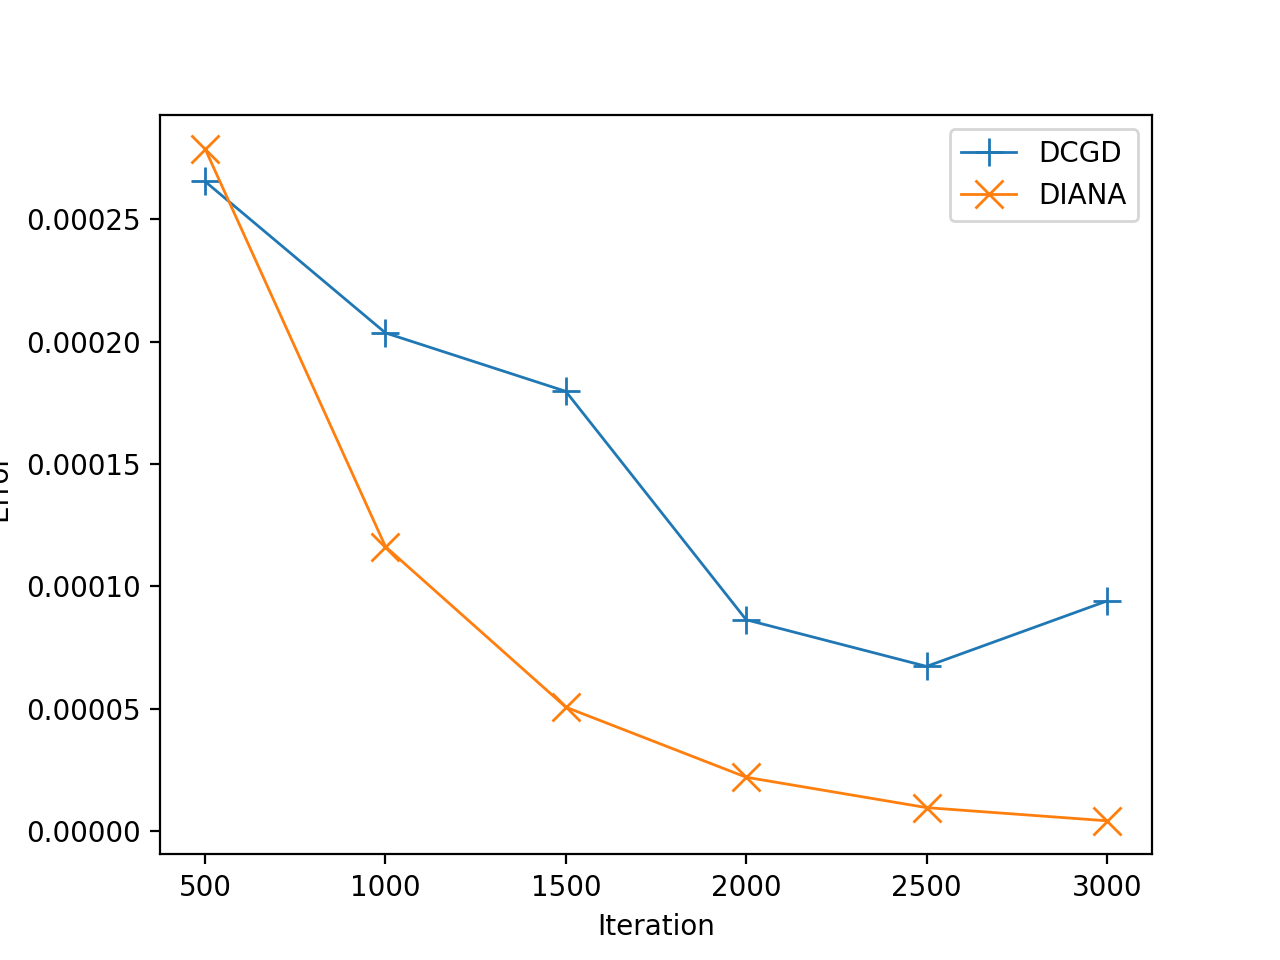
\includegraphics[width=6.7cm]{Figure_71.png}} 
		\subfigure[]{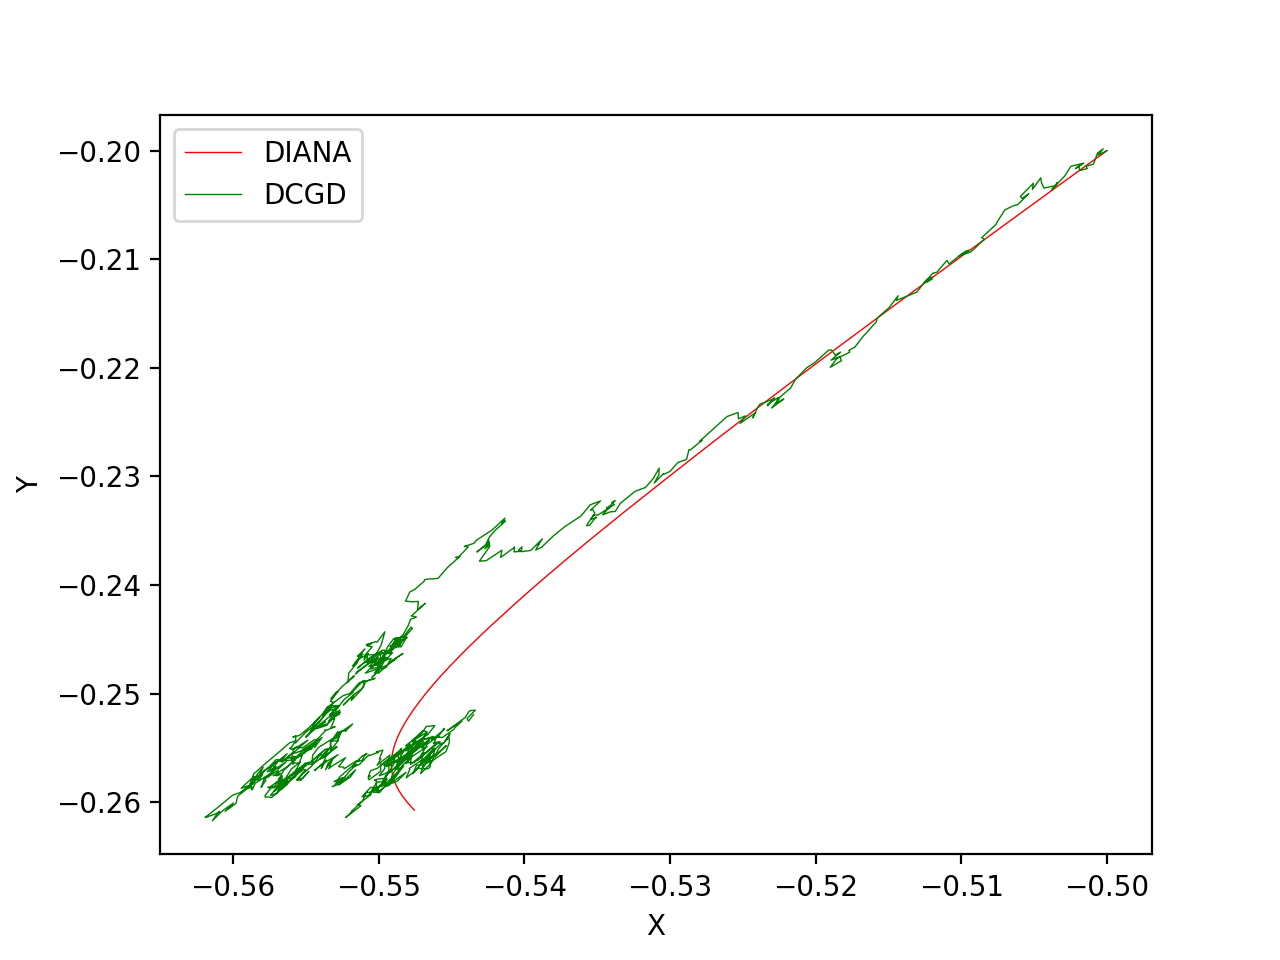
\includegraphics[width=6.7cm]{Figure_72.png}}
	
		
		\caption{ (a) shows the error in terms of iteration,(b)  shows the trajectories of DINANA and DCGD, you can see that DCGD will converge to the neighborhood of  the optimal point with fluctuation while DIANA converges to the optimal point very smoothly, this quite matches the theory's prediction.} %图片标题
		\label{img2}
	\end{figure}
	
	
	
	
	\paragraph{p2.}	(i)
	\begin{equation}
		g^k=\frac{1}{\tau}\sum_{i\in S^k}(\nabla f_i(x^k)-\nabla f_i(w_i^k))+\frac{1}{n}\sum_{j=1}^{n}\nabla f_j(w_j^k)
	\end{equation}
	\begin{equation}
		w_{j}^{k+1}= \begin{cases}x^{k} & j\in S^k\\ w_{j}^{k} & else \end{cases}
	\end{equation}	
	(ii)
	\begin{lemma}
		Assume that for each $i=1,2, \ldots, n$, the function $f_{i}$ is convex and $L_{i}$-smooth. Then for SAGA-NICE, we have the following recursions:
		$$
		\mathrm{E}\left[\left\|g^{k}-\nabla f\left(x^{\star}\right)\right\|^{2} \mid x^{k}, w^{k}\right] \leq 2 \underbrace{\left(2 \left(\frac{n-\tau}{\tau(n-1)} \max _{i} L_{i}+\frac{n(\tau-1)}{\tau(n-1)} L\right) \right)}_{A} D_{f}\left(x^{k}, x^{\star}\right)+\underbrace{2}_{B} \sigma^{k}
		$$
		and
		$$
		\mathrm{E}\left[\sigma^{k+1} \mid x^{k}, w^{k}\right] \leq 2 \underbrace{\frac{\tau L_{\max }}{n}}_{\tilde{A}} D_{f}\left(x^{k}, x^{\star}\right)+\underbrace{\left(1-\frac{\tau}{n}\right)}_{\tilde{B}} \sigma^{k}
		$$
		where $\sigma(w) \stackrel{\text { def }}{=} \frac{1}{n} \sum_{i=1}^{n}\left\|\nabla f_{i}\left(w_{i}\right)-\nabla f_{i}\left(x^{\star}\right)\right\|^{2}$ and
		$$
		\sigma^{k} \stackrel{\text { def }}{=} \sigma\left(w^{k}\right)=\frac{1}{n} \sum^{n}\left\|\nabla f_{i}\left(w_{i}^{k}\right)-\nabla f_{i}\left(x^{\star}\right)\right\|^{2}
		$$
	\end{lemma}
	\begin{proof}
		\begin{equation}
			\begin{aligned}
				&\E\left[||g^k-\nabla f(x^{\star})||^2\mid x^k,w^k\right]\\
				&=\mathrm{E}\left[\left\|\frac{1}{\tau}\sum_{i\in S^k}\nabla f_{i}\left(w^{k}\right)-\nabla f_{i}\left(w_{i}^{k}\right)+\frac{1}{n} \frac{1}{\tau}\sum_{j=1}^{n} \nabla f_{j}\left(w_{j}^{k}\right)-\nabla f\left(x^{\star}\right)\right\|^{2} \mid x^{k}, w^{k}\right]\\
				&=\mathrm{E}\left[\left\|\frac{1}{\tau}\sum_{i\in S^k}\nabla f_{i}\left(x^{k}\right)-\nabla f_{i}\left(x^{\star}\right)+\nabla f_{i}\left(x^{\star}\right)-\nabla f_{i}\left(w_{i}^{k}\right)+\frac{1}{n} \sum_{j=1}^{n} \nabla f_{j}\left(w_{j}^{k}\right)-\nabla f\left(x^{\star}\right)\right\|^{2} \mid x^{k}, w^{k}\right]\\
				&\leq E\left[2\left\|\frac{1}{\tau}\sum_{i\in S^k}\nabla f_{i}\left(x^{k}\right)-\nabla f_{i}\left(x^{\star}\right)\right\|^{2} \mid x^{k}, w^{k}\right]\\
				&+\mathrm{E}\left[2\left\|\frac{1}{\tau}\sum_{i\in S^k}\nabla f_{i}\left(x^{\star}\right)-\nabla f_{i}\left(w_{i}^{k}\right)+\frac{1}{n} \sum_{j=1}^{n} \nabla f_{j}\left(w_{j}^{k}\right)-\nabla f\left(x^{\star}\right)\right \|^{2} \mid x^{k}, w^{k}\right]\\
				&=2 \mathrm{E}\left[\left\|\frac{1}{\tau}\sum_{i\in S^k}\nabla f_{i}\left(x^{k}\right)-\nabla f_{i}\left(x^{\star}\right)\right\|^{2} \mid x^{k}, w^{k}\right]\\
				&+2 \mathrm{E}\left[\|\underbrace{\frac{1}{\tau}\sum_{i\in S^k}\nabla f_{i}\left(x^{\star}\right)-\nabla f_{i}\left(w_{i}^{k}\right)}_{A_{i}}-\underbrace{\left(\nabla f\left(x^{\star}\right)-\frac{1}{n} \sum_{j=1}^{n} \nabla f_{j}\left(w_{j}^{k}\right)\right)}_{\mathrm{E}\left[A_{i} \mid x^{k}, w^{k}\right]}\|^{2} \mid x^{k}, w^{k}\right] .
			\end{aligned}
		\end{equation}
	Applying the inequality
	$$
	\mathrm{E}\left[\left\|A_{i}-\mathrm{E}\left[A_{i} \mid x^{k}, w^{k}\right]\right\|^{2} \mid x^{k}, w^{k}\right] \leq \mathrm{E}\left[\left\|A_{i}\right\|^{2} \mid x^{k}, w^{k}\right]
	$$
	we can continue
	\begin{equation}
		\begin{aligned}
			&\mathrm{E}\left[\left\|g^{k}-\nabla f\left(x^{\star}\right)\right\|^{2} \mid x^{k}, w^{k}\right] \\
			&\leq 2 \mathrm{E}\left[\left\|\frac{1}{\tau}\sum_{i\in S^k}\nabla f_{i}\left(x^{k}\right)-\nabla f_{i}\left(x^{\star}\right)\right\|^{2} \mid x^{k}, w^{k}\right] +2 \mathrm{E}\left[\left\|\frac{1}{\tau}\sum_{i\in S^k}\nabla f_{i}\left(x^{\star}\right)-\nabla f_{i}\left(w_{i}^{k}\right)\right\|^{2} \mid x^{k}, w^{k}\right] \\
			&=2 (\frac{n-\tau}{\tau(n-1)}\frac{1}{n}\sum_{i=1}^n||\nabla f_i(x^k)-\nabla f_i(x^{\star})||^2+\frac{n(\tau-1)}{\tau(n-1)}||\nabla f(x^k)-\nabla f(x^{\star})||^2)\\
			&+2 (\frac{n-\tau}{\tau(n-1)}\frac{1}{n}\sum_{i=1}^n||\nabla f_i(x^{\star})-\nabla f_i(w^k_i)||^2+\frac{n(\tau-1)}{\tau(n-1)}||\frac{1}{n}\sum_{i=1}^{n}\nabla f_i(w^k_i)-\nabla f_i(x^{\star})||^2)\\
			&\leq 2 (\frac{n-\tau}{\tau(n-1)}\frac{1}{n}\sum_{i=1}^n||\nabla f_i(x^k)-\nabla f_i(x^{\star})||^2+\frac{n(\tau-1)}{\tau(n-1)}||\nabla f(x^k)-\nabla f(x^{\star})||^2)\\
			&+2 (\frac{n-\tau}{\tau(n-1)}\frac{1}{n}\sum_{i=1}^n||\nabla f_i(x^{\star})-\nabla f_i(w^k_i)||^2+\frac{n(\tau-1)}{\tau(n-1)}\frac{1}{n}\sum_{i=1}^{n}||\nabla f_i(w^k_i)-\nabla f_i(x^{\star})||^2)\\
			&= 2 (\frac{n-\tau}{\tau(n-1)}\frac{1}{n}\sum_{i=1}^n||\nabla f_i(x^k)-\nabla f_i(x^{\star})||^2+\frac{n(\tau-1)}{\tau(n-1)}||\nabla f(x^k)-\nabla f(x^{\star})||^2)\\
			&+2\frac{1}{n} \sum_{i=1}^n||\nabla f_i(x^{\star})-\nabla f_i(w^k_i)||^2\\
			& \leq 4\left(\frac{n-\tau}{\tau(n-1)} \max _{i} L_{i}+\frac{n(\tau-1)}{\tau(n-1)} L\right) D_{f}(x^k, x^{\star})+2\sigma^k
		\end{aligned}
	\end{equation}
We now proceed to the second recursion. First, note that for every $i$ we have
$$
w_{i}^{k+1}=\left\{\begin{array}{lll}
	w_{i}^{k} & \text { with probability } & 1-\frac{\tau}{n} \\
	x^{k} & \text { with probability } & \frac{\tau}{n}
\end{array}\right.
$$
Therefore,
$$
\begin{aligned}
	\mathrm{E}\left[\sigma^{k+1} \mid x^{k}, w^{k}\right] &=\frac{1}{n} \sum_{i=1}^{n} \mathrm{E}\left[\left\|\nabla f_{i}\left(w_{i}^{k+1}\right)-\nabla f_{i}\left(x^{\star}\right)\right\|^{2} \mid x^{k}, w^{k}\right] \\
	& \stackrel{}{=} \frac{1}{n} \sum_{i=1}^{n}\left[\left(1-\frac{\tau}{n}\right)\left\|\nabla f_{i}\left(w_{i}^{k}\right)-\nabla f_{i}\left(x^{\star}\right)\right\|^{2}+\frac{\tau}{n}\left\|\nabla f_{i}\left(x^{k}\right)-\nabla f_{i}\left(x^{\star}\right)\right\|^{2}\right] \\
	&=\left(1-\frac{\tau}{n}\right) \sigma^{k}+\frac{\tau}{n^{2}} \sum_{i=1}^{n} \underbrace{\left\|\nabla f_{i}\left(x^{k}\right)-\nabla f_{i}\left(x^{\star}\right)\right\|^{2}}_{\leq 2 L_{i} D_{f_{i}}\left(x^{k}, x^{\star}\right)} \\
	& \leq\left(1-\frac{\tau}{n}\right) \sigma^{k}+\frac{2\tau L_{\max }}{n} D_{f}\left(x^{k}, x^{\star}\right)
\end{aligned}
$$
	\end{proof}
	$\sigma^k$ is the same as in the lecture.
	\newline
	(iii)
	\begin{corollary}
		Assume that for each $i$, the function $f_{i}$ is convex $L_{i}$-smooth. Further assume $f$ is $\mu$-convex. Choose $\gamma=\frac{1}{6 L_{\max }}$. Then SAGA-NICE satisfies:
		$$
		\mathrm{E}\left[V^{k}\right] \leq\left(1-\min \left\{\frac{\mu}{6 L_{\max }}, \frac{\tau}{2 n}\right\}\right)^{k} V^{0}
		$$
		where the Lyapunov function is defined by
		$$
		V^{k} \stackrel{\text { def }}{=}\left\|x^{k}-x^{\star}\right\|^{2}+\frac{n}{9\tau L_{\max }^{2}} \sigma^{k}
		$$
		and
		$$
		\sigma^{k} \stackrel{\text { def }}{=} \frac{1}{n} \sum_{i=1}^{n}\left\|\nabla f_{i}\left(w_{i}^{k}\right)-\nabla f_{i}\left(x^{\star}\right)\right\|^{2}
		$$
	\end{corollary}
\begin{proof}
	In view of (ii), Assumption 6 holds with
	$$
	A\leq 2 L_{\max }, \quad B=2, \quad \tilde{A}=\frac{\tau L_{\max }}{n}, \quad \tilde{B}=1-\frac{\tau}{n}, \quad C=\tilde{C}=0
	$$
	
	We can now apply Theorem 94 with $M=\frac{4n}{\tau}>\frac{2n}{\tau}=\frac{B}{1-\tilde{B}} .$ Note that
	$$
	A+M \tilde{A}=(2+\frac{4}{\tau}) L_{\max }>\mu
	$$
	and hence the stepsize bound becomes
	$$
	0<\gamma \leq \min \left\{\frac{1}{\mu}, \frac{1}{A+M \tilde{A}}\right\}=\frac{1}{A+M \tilde{A}}=\frac{1}{6 L_{\max }}
	$$
	So, the choice $\gamma=\frac{1}{6 L_{\max }}$ is justified. Since $\frac{B+M \tilde{B}}{M}=1+\frac{2}{4 n}-\frac{1}{n}=1-\frac{\tau}{2 n}$ and using $\gamma=\frac{1}{6 L_{\max }}$, the rate in Theorem 94 becomes
	$$
	\begin{aligned}
		\max \left\{(1-\gamma \mu)^{k},\left(\frac{B+M \tilde{B}}{M}\right)^{k}\right\} &=\max \left\{\left(1-\frac{\mu}{6 L_{\max }}\right)^{k},\left(1-\frac{\tau}{2 n}\right)^{k}\right\} \\
		&=\left(1-\min \left\{\frac{\mu}{6 L_{\max }}, \frac{\tau}{2 n}\right\}\right)^{k}
	\end{aligned}
	$$
	Finally, the Lyapunov function is
	$$
	V^{k}=\left\|x^{k}-x^{\star}\right\|^{2}+M \gamma^{2} \sigma^{k}=\left\|x^{k}-x^{\star}\right\|^{2} \frac{4 n}{\tau36 L_{\max }^{2}} \sigma^{k}
	$$
\end{proof}
so
$$
k \geq \max \left\{\frac{6 L_{\max }}{\mu}, \frac{2n}{\tau}\right\} \log \frac{1}{\varepsilon} \Rightarrow \mathrm{E}\left[V^{k}\right] \leq \varepsilon V^{0}
$$.
(the step size here chosen is not the best).
\newline	
(iv)
when $\tau=1$, lemma in (ii) is exactly lemma 103. when $\tau = n$, then this is gradient descent, rate from (iii) is
$$
k \geq \max \left\{\frac{6 L_{\max }}{\mu}, 2\right\} \log \frac{1}{\varepsilon} =\frac{6 L_{\max }}{\mu}\log \frac{1}{\varepsilon}\Rightarrow \mathrm{E}\left[V^{k}\right] \leq \varepsilon V^{0}
$$, here the rate involves $L_{max}$ instead of $L$.
	
	
	
	
	
	
	
	
	
	
	
	
	
	
	
	
	
	
	
	
	
	
	
	
	
	
	
	
	
	
	
	
	
	
\end{document}